\parbox{.5\textwidth}{\begin{tabular}{ll|r}
\multicolumn{3}{l}{NA20278, AFR, ASW}\\ \hline\rule[-1ex]{0cm}{4ex}EURO & ad \hspace{1cm} \parbox{.5cm}{$q$ \\[-1.3ex] \mbox{}}& 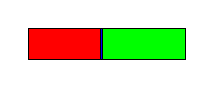
\begin{tikzpicture} 
\draw[fill=red] (0cm, 0cm) rectangle (0.916cm, .4cm);
\draw[fill=blue] (0.916cm, 0cm) rectangle (0.938cm, .4cm);
\draw[fill=green] (0.938cm, 0cm) rectangle (2cm, .4cm);
\draw[fill=yellow] (2cm, 0cm) rectangle (2cm, .4cm);
\end{tikzpicture}
\\ \cline{2-3}
\rule[-3ex]{0cm}{7ex} $\Delta\ell =$  6.69 & r-ad \hspace{0cm} \parbox{1cm}{\hfill $q^{MP}$ \ $q^M, q^P$} & \parbox{2cm}{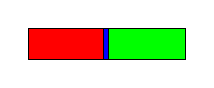
\begin{tikzpicture} 
\draw[fill=red] (0cm, 0cm) rectangle (0.96cm, .4cm);
\draw[fill=blue] (0.96cm, 0cm) rectangle (1.014cm, .4cm);
\draw[fill=green] (1.014cm, 0cm) rectangle (2cm, .4cm);
\draw[fill=yellow] (2cm, 0cm) rectangle (2cm, .4cm);
\end{tikzpicture}
\\[-1.3ex]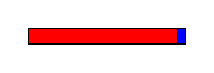
\begin{tikzpicture} 
\draw[fill=red] (0cm, 0cm) rectangle (1.894cm, .2cm);
\draw[fill=blue] (1.894cm, 0cm) rectangle (2cm, .2cm);
\draw[fill=green] (2cm, 0cm) rectangle (2cm, .2cm);
\draw[fill=yellow] (2cm, 0cm) rectangle (2cm, .2cm);
\end{tikzpicture}
\\[-2ex]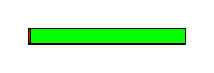
\begin{tikzpicture} 
\draw[fill=red] (0cm, 0cm) rectangle (0.028cm, .2cm);
\draw[fill=blue] (0.028cm, 0cm) rectangle (0.028cm, .2cm);
\draw[fill=green] (0.028cm, 0cm) rectangle (2cm, .2cm);
\draw[fill=yellow] (2cm, 0cm) rectangle (2cm, .2cm);
\end{tikzpicture}
}\\ \hline 
\rule[-1ex]{0cm}{4ex}Kidd & ad \hspace{1cm} \parbox{.5cm}{$q$ \\[-1.3ex] \mbox{}}& 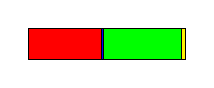
\begin{tikzpicture} 
\draw[fill=red] (0cm, 0cm) rectangle (0.934cm, .4cm);
\draw[fill=blue] (0.934cm, 0cm) rectangle (0.954cm, .4cm);
\draw[fill=green] (0.954cm, 0cm) rectangle (1.948cm, .4cm);
\draw[fill=yellow] (1.948cm, 0cm) rectangle (2cm, .4cm);
\end{tikzpicture}
 \\ \cline{2-3}
\rule[-3ex]{0cm}{7ex}$\Delta\ell =$  9.98  & r-ad \hspace{0cm} \parbox{1cm}{\hfill $q^{MP}$ \ $q^M, q^P$} & \parbox{2cm}{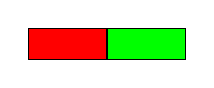
\begin{tikzpicture} 
\draw[fill=red] (0cm, 0cm) rectangle (1cm, .4cm);
\draw[fill=blue] (1cm, 0cm) rectangle (1cm, .4cm);
\draw[fill=green] (1cm, 0cm) rectangle (2cm, .4cm);
\draw[fill=yellow] (2cm, 0cm) rectangle (2cm, .4cm);
\end{tikzpicture}
\\[-1.3ex]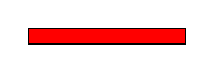
\begin{tikzpicture} 
\draw[fill=red] (0cm, 0cm) rectangle (2cm, .2cm);
\draw[fill=blue] (2cm, 0cm) rectangle (2cm, .2cm);
\draw[fill=green] (2cm, 0cm) rectangle (2cm, .2cm);
\draw[fill=yellow] (2cm, 0cm) rectangle (2cm, .2cm);
\end{tikzpicture}
\\[-2ex]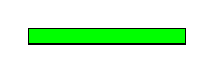
\begin{tikzpicture} 
\draw[fill=red] (0cm, 0cm) rectangle (0cm, .2cm);
\draw[fill=blue] (0cm, 0cm) rectangle (0cm, .2cm);
\draw[fill=green] (0cm, 0cm) rectangle (2cm, .2cm);
\draw[fill=yellow] (2cm, 0cm) rectangle (2cm, .2cm);
\end{tikzpicture}
}\\ \hline 
\end{tabular}}\parbox{.5\textwidth}{\begin{tabular}{ll|r}
\multicolumn{3}{l}{NA20342, AFR, ASW}\\ \hline\rule[-1ex]{0cm}{4ex}EURO & ad \hspace{1cm} \parbox{.5cm}{$q$ \\[-1.3ex] \mbox{}}& 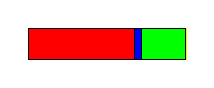
\begin{tikzpicture} 
\draw[fill=red] (0cm, 0cm) rectangle (1.35cm, .4cm);
\draw[fill=blue] (1.35cm, 0cm) rectangle (1.434cm, .4cm);
\draw[fill=green] (1.434cm, 0cm) rectangle (1.998cm, .4cm);
\draw[fill=yellow] (1.998cm, 0cm) rectangle (2cm, .4cm);
\end{tikzpicture}
\\ \cline{2-3}
\rule[-3ex]{0cm}{7ex} $\Delta\ell =$  1.82 & r-ad \hspace{0cm} \parbox{1cm}{\hfill $q^{MP}$ \ $q^M, q^P$} & \parbox{2cm}{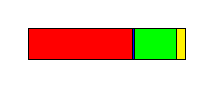
\begin{tikzpicture} 
\draw[fill=red] (0cm, 0cm) rectangle (1.32cm, .4cm);
\draw[fill=blue] (1.32cm, 0cm) rectangle (1.354cm, .4cm);
\draw[fill=green] (1.354cm, 0cm) rectangle (1.886cm, .4cm);
\draw[fill=yellow] (1.886cm, 0cm) rectangle (2cm, .4cm);
\end{tikzpicture}
\\[-1.3ex]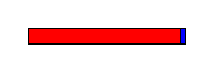
\begin{tikzpicture} 
\draw[fill=red] (0cm, 0cm) rectangle (1.938cm, .2cm);
\draw[fill=blue] (1.938cm, 0cm) rectangle (2cm, .2cm);
\draw[fill=green] (2cm, 0cm) rectangle (2cm, .2cm);
\draw[fill=yellow] (2cm, 0cm) rectangle (2cm, .2cm);
\end{tikzpicture}
\\[-2ex]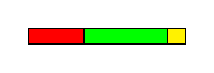
\begin{tikzpicture} 
\draw[fill=red] (0cm, 0cm) rectangle (0.702cm, .2cm);
\draw[fill=blue] (0.702cm, 0cm) rectangle (0.708cm, .2cm);
\draw[fill=green] (0.708cm, 0cm) rectangle (1.772cm, .2cm);
\draw[fill=yellow] (1.772cm, 0cm) rectangle (2cm, .2cm);
\end{tikzpicture}
}\\ \hline 
\rule[-1ex]{0cm}{4ex}Kidd & ad \hspace{1cm} \parbox{.5cm}{$q$ \\[-1.3ex] \mbox{}}& 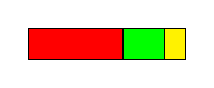
\begin{tikzpicture} 
\draw[fill=red] (0cm, 0cm) rectangle (1.204cm, .4cm);
\draw[fill=blue] (1.204cm, 0cm) rectangle (1.204cm, .4cm);
\draw[fill=green] (1.204cm, 0cm) rectangle (1.732cm, .4cm);
\draw[fill=yellow] (1.732cm, 0cm) rectangle (2cm, .4cm);
\end{tikzpicture}
 \\ \cline{2-3}
\rule[-3ex]{0cm}{7ex}$\Delta\ell =$  3.66  & r-ad \hspace{0cm} \parbox{1cm}{\hfill $q^{MP}$ \ $q^M, q^P$} & \parbox{2cm}{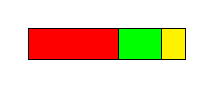
\begin{tikzpicture} 
\draw[fill=red] (0cm, 0cm) rectangle (1.144cm, .4cm);
\draw[fill=blue] (1.144cm, 0cm) rectangle (1.144cm, .4cm);
\draw[fill=green] (1.144cm, 0cm) rectangle (1.692cm, .4cm);
\draw[fill=yellow] (1.692cm, 0cm) rectangle (2cm, .4cm);
\end{tikzpicture}
\\[-1.3ex]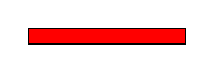
\begin{tikzpicture} 
\draw[fill=red] (0cm, 0cm) rectangle (2cm, .2cm);
\draw[fill=blue] (2cm, 0cm) rectangle (2cm, .2cm);
\draw[fill=green] (2cm, 0cm) rectangle (2cm, .2cm);
\draw[fill=yellow] (2cm, 0cm) rectangle (2cm, .2cm);
\end{tikzpicture}
\\[-2ex]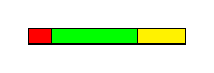
\begin{tikzpicture} 
\draw[fill=red] (0cm, 0cm) rectangle (0.29cm, .2cm);
\draw[fill=blue] (0.29cm, 0cm) rectangle (0.29cm, .2cm);
\draw[fill=green] (0.29cm, 0cm) rectangle (1.386cm, .2cm);
\draw[fill=yellow] (1.386cm, 0cm) rectangle (2cm, .2cm);
\end{tikzpicture}
}\\ \hline 
\end{tabular}} 

\vspace{2ex}\parbox{.5\textwidth}{\begin{tabular}{ll|r}
\multicolumn{3}{l}{NA20274, AFR, ASW}\\ \hline\rule[-1ex]{0cm}{4ex}EURO & ad \hspace{1cm} \parbox{.5cm}{$q$ \\[-1.3ex] \mbox{}}& 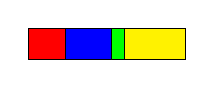
\begin{tikzpicture} 
\draw[fill=red] (0cm, 0cm) rectangle (0.478cm, .4cm);
\draw[fill=blue] (0.478cm, 0cm) rectangle (1.056cm, .4cm);
\draw[fill=green] (1.056cm, 0cm) rectangle (1.222cm, .4cm);
\draw[fill=yellow] (1.222cm, 0cm) rectangle (2cm, .4cm);
\end{tikzpicture}
\\ \cline{2-3}
\rule[-3ex]{0cm}{7ex} $\Delta\ell =$  6.56 & r-ad \hspace{0cm} \parbox{1cm}{\hfill $q^{MP}$ \ $q^M, q^P$} & \parbox{2cm}{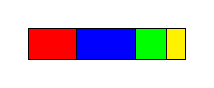
\begin{tikzpicture} 
\draw[fill=red] (0cm, 0cm) rectangle (0.61cm, .4cm);
\draw[fill=blue] (0.61cm, 0cm) rectangle (1.368cm, .4cm);
\draw[fill=green] (1.368cm, 0cm) rectangle (1.758cm, .4cm);
\draw[fill=yellow] (1.758cm, 0cm) rectangle (2cm, .4cm);
\end{tikzpicture}
\\[-1.3ex]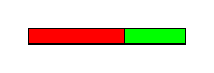
\begin{tikzpicture} 
\draw[fill=red] (0cm, 0cm) rectangle (1.222cm, .2cm);
\draw[fill=blue] (1.222cm, 0cm) rectangle (1.222cm, .2cm);
\draw[fill=green] (1.222cm, 0cm) rectangle (2cm, .2cm);
\draw[fill=yellow] (2cm, 0cm) rectangle (2cm, .2cm);
\end{tikzpicture}
\\[-2ex]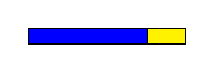
\begin{tikzpicture} 
\draw[fill=red] (0cm, 0cm) rectangle (0cm, .2cm);
\draw[fill=blue] (0cm, 0cm) rectangle (1.514cm, .2cm);
\draw[fill=green] (1.514cm, 0cm) rectangle (1.514cm, .2cm);
\draw[fill=yellow] (1.514cm, 0cm) rectangle (2cm, .2cm);
\end{tikzpicture}
}\\ \hline 
\rule[-1ex]{0cm}{4ex}Kidd & ad \hspace{1cm} \parbox{.5cm}{$q$ \\[-1.3ex] \mbox{}}& 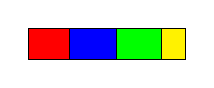
\begin{tikzpicture} 
\draw[fill=red] (0cm, 0cm) rectangle (0.528cm, .4cm);
\draw[fill=blue] (0.528cm, 0cm) rectangle (1.118cm, .4cm);
\draw[fill=green] (1.118cm, 0cm) rectangle (1.696cm, .4cm);
\draw[fill=yellow] (1.696cm, 0cm) rectangle (2cm, .4cm);
\end{tikzpicture}
 \\ \cline{2-3}
\rule[-3ex]{0cm}{7ex}$\Delta\ell =$  2.68  & r-ad \hspace{0cm} \parbox{1cm}{\hfill $q^{MP}$ \ $q^M, q^P$} & \parbox{2cm}{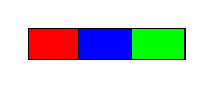
\begin{tikzpicture} 
\draw[fill=red] (0cm, 0cm) rectangle (0.636cm, .4cm);
\draw[fill=blue] (0.636cm, 0cm) rectangle (1.31cm, .4cm);
\draw[fill=green] (1.31cm, 0cm) rectangle (1.99cm, .4cm);
\draw[fill=yellow] (1.99cm, 0cm) rectangle (2cm, .4cm);
\end{tikzpicture}
\\[-1.3ex]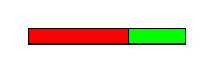
\begin{tikzpicture} 
\draw[fill=red] (0cm, 0cm) rectangle (1.272cm, .2cm);
\draw[fill=blue] (1.272cm, 0cm) rectangle (1.272cm, .2cm);
\draw[fill=green] (1.272cm, 0cm) rectangle (2cm, .2cm);
\draw[fill=yellow] (2cm, 0cm) rectangle (2cm, .2cm);
\end{tikzpicture}
\\[-2ex]
\begin{tikzpicture} 
\draw[fill=red] (0cm, 0cm) rectangle (0cm, .2cm);
\draw[fill=blue] (0cm, 0cm) rectangle (1.348cm, .2cm);
\draw[fill=green] (1.348cm, 0cm) rectangle (1.982cm, .2cm);
\draw[fill=yellow] (1.982cm, 0cm) rectangle (2cm, .2cm);
\end{tikzpicture}
}\\ \hline 
\end{tabular}}\parbox{.5\textwidth}{\begin{tabular}{ll|r}
\multicolumn{3}{l}{NA19625, AFR, ASW}\\ \hline\rule[-1ex]{0cm}{4ex}EURO & ad \hspace{1cm} \parbox{.5cm}{$q$ \\[-1.3ex] \mbox{}}& 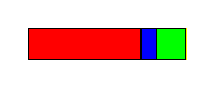
\begin{tikzpicture} 
\draw[fill=red] (0cm, 0cm) rectangle (1.432cm, .4cm);
\draw[fill=blue] (1.432cm, 0cm) rectangle (1.634cm, .4cm);
\draw[fill=green] (1.634cm, 0cm) rectangle (1.998cm, .4cm);
\draw[fill=yellow] (1.998cm, 0cm) rectangle (2cm, .4cm);
\end{tikzpicture}
\\ \cline{2-3}
\rule[-3ex]{0cm}{7ex} $\Delta\ell =$  1.52 & r-ad \hspace{0cm} \parbox{1cm}{\hfill $q^{MP}$ \ $q^M, q^P$} & \parbox{2cm}{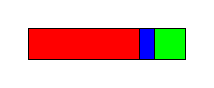
\begin{tikzpicture} 
\draw[fill=red] (0cm, 0cm) rectangle (1.41cm, .4cm);
\draw[fill=blue] (1.41cm, 0cm) rectangle (1.608cm, .4cm);
\draw[fill=green] (1.608cm, 0cm) rectangle (2cm, .4cm);
\draw[fill=yellow] (2cm, 0cm) rectangle (2cm, .4cm);
\end{tikzpicture}
\\[-1.3ex]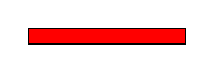
\begin{tikzpicture} 
\draw[fill=red] (0cm, 0cm) rectangle (2cm, .2cm);
\draw[fill=blue] (2cm, 0cm) rectangle (2cm, .2cm);
\draw[fill=green] (2cm, 0cm) rectangle (2cm, .2cm);
\draw[fill=yellow] (2cm, 0cm) rectangle (2cm, .2cm);
\end{tikzpicture}
\\[-2ex]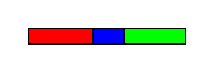
\begin{tikzpicture} 
\draw[fill=red] (0cm, 0cm) rectangle (0.822cm, .2cm);
\draw[fill=blue] (0.822cm, 0cm) rectangle (1.216cm, .2cm);
\draw[fill=green] (1.216cm, 0cm) rectangle (2cm, .2cm);
\draw[fill=yellow] (2cm, 0cm) rectangle (2cm, .2cm);
\end{tikzpicture}
}\\ \hline 
\rule[-1ex]{0cm}{4ex}Kidd & ad \hspace{1cm} \parbox{.5cm}{$q$ \\[-1.3ex] \mbox{}}& 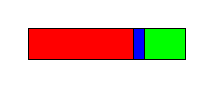
\begin{tikzpicture} 
\draw[fill=red] (0cm, 0cm) rectangle (1.342cm, .4cm);
\draw[fill=blue] (1.342cm, 0cm) rectangle (1.482cm, .4cm);
\draw[fill=green] (1.482cm, 0cm) rectangle (2cm, .4cm);
\draw[fill=yellow] (2cm, 0cm) rectangle (2cm, .4cm);
\end{tikzpicture}
 \\ \cline{2-3}
\rule[-3ex]{0cm}{7ex}$\Delta\ell =$  1.6  & r-ad \hspace{0cm} \parbox{1cm}{\hfill $q^{MP}$ \ $q^M, q^P$} & \parbox{2cm}{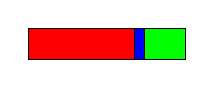
\begin{tikzpicture} 
\draw[fill=red] (0cm, 0cm) rectangle (1.352cm, .4cm);
\draw[fill=blue] (1.352cm, 0cm) rectangle (1.472cm, .4cm);
\draw[fill=green] (1.472cm, 0cm) rectangle (2cm, .4cm);
\draw[fill=yellow] (2cm, 0cm) rectangle (2cm, .4cm);
\end{tikzpicture}
\\[-1.3ex]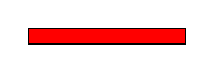
\begin{tikzpicture} 
\draw[fill=red] (0cm, 0cm) rectangle (2cm, .2cm);
\draw[fill=blue] (2cm, 0cm) rectangle (2cm, .2cm);
\draw[fill=green] (2cm, 0cm) rectangle (2cm, .2cm);
\draw[fill=yellow] (2cm, 0cm) rectangle (2cm, .2cm);
\end{tikzpicture}
\\[-2ex]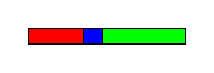
\begin{tikzpicture} 
\draw[fill=red] (0cm, 0cm) rectangle (0.704cm, .2cm);
\draw[fill=blue] (0.704cm, 0cm) rectangle (0.944cm, .2cm);
\draw[fill=green] (0.944cm, 0cm) rectangle (2cm, .2cm);
\draw[fill=yellow] (2cm, 0cm) rectangle (2cm, .2cm);
\end{tikzpicture}
}\\ \hline 
\end{tabular}} 

\vspace{2ex}\parbox{.5\textwidth}{\begin{tabular}{ll|r}
\multicolumn{3}{l}{NA20355, AFR, ASW}\\ \hline\rule[-1ex]{0cm}{4ex}EURO & ad \hspace{1cm} \parbox{.5cm}{$q$ \\[-1.3ex] \mbox{}}& 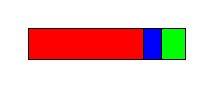
\begin{tikzpicture} 
\draw[fill=red] (0cm, 0cm) rectangle (1.462cm, .4cm);
\draw[fill=blue] (1.462cm, 0cm) rectangle (1.698cm, .4cm);
\draw[fill=green] (1.698cm, 0cm) rectangle (2cm, .4cm);
\draw[fill=yellow] (2cm, 0cm) rectangle (2cm, .4cm);
\end{tikzpicture}
\\ \cline{2-3}
\rule[-3ex]{0cm}{7ex} $\Delta\ell =$  1.11 & r-ad \hspace{0cm} \parbox{1cm}{\hfill $q^{MP}$ \ $q^M, q^P$} & \parbox{2cm}{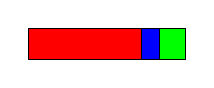
\begin{tikzpicture} 
\draw[fill=red] (0cm, 0cm) rectangle (1.438cm, .4cm);
\draw[fill=blue] (1.438cm, 0cm) rectangle (1.67cm, .4cm);
\draw[fill=green] (1.67cm, 0cm) rectangle (2cm, .4cm);
\draw[fill=yellow] (2cm, 0cm) rectangle (2cm, .4cm);
\end{tikzpicture}
\\[-1.3ex]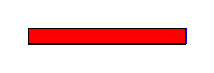
\begin{tikzpicture} 
\draw[fill=red] (0cm, 0cm) rectangle (1.998cm, .2cm);
\draw[fill=blue] (1.998cm, 0cm) rectangle (2cm, .2cm);
\draw[fill=green] (2cm, 0cm) rectangle (2cm, .2cm);
\draw[fill=yellow] (2cm, 0cm) rectangle (2cm, .2cm);
\end{tikzpicture}
\\[-2ex]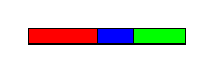
\begin{tikzpicture} 
\draw[fill=red] (0cm, 0cm) rectangle (0.878cm, .2cm);
\draw[fill=blue] (0.878cm, 0cm) rectangle (1.34cm, .2cm);
\draw[fill=green] (1.34cm, 0cm) rectangle (2cm, .2cm);
\draw[fill=yellow] (2cm, 0cm) rectangle (2cm, .2cm);
\end{tikzpicture}
}\\ \hline 
\rule[-1ex]{0cm}{4ex}Kidd & ad \hspace{1cm} \parbox{.5cm}{$q$ \\[-1.3ex] \mbox{}}& 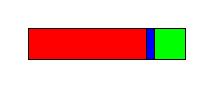
\begin{tikzpicture} 
\draw[fill=red] (0cm, 0cm) rectangle (1.498cm, .4cm);
\draw[fill=blue] (1.498cm, 0cm) rectangle (1.602cm, .4cm);
\draw[fill=green] (1.602cm, 0cm) rectangle (2cm, .4cm);
\draw[fill=yellow] (2cm, 0cm) rectangle (2cm, .4cm);
\end{tikzpicture}
 \\ \cline{2-3}
\rule[-3ex]{0cm}{7ex}$\Delta\ell =$  1.55  & r-ad \hspace{0cm} \parbox{1cm}{\hfill $q^{MP}$ \ $q^M, q^P$} & \parbox{2cm}{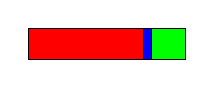
\begin{tikzpicture} 
\draw[fill=red] (0cm, 0cm) rectangle (1.464cm, .4cm);
\draw[fill=blue] (1.464cm, 0cm) rectangle (1.56cm, .4cm);
\draw[fill=green] (1.56cm, 0cm) rectangle (2cm, .4cm);
\draw[fill=yellow] (2cm, 0cm) rectangle (2cm, .4cm);
\end{tikzpicture}
\\[-1.3ex]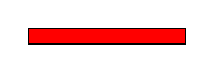
\begin{tikzpicture} 
\draw[fill=red] (0cm, 0cm) rectangle (2cm, .2cm);
\draw[fill=blue] (2cm, 0cm) rectangle (2cm, .2cm);
\draw[fill=green] (2cm, 0cm) rectangle (2cm, .2cm);
\draw[fill=yellow] (2cm, 0cm) rectangle (2cm, .2cm);
\end{tikzpicture}
\\[-2ex]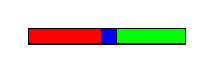
\begin{tikzpicture} 
\draw[fill=red] (0cm, 0cm) rectangle (0.928cm, .2cm);
\draw[fill=blue] (0.928cm, 0cm) rectangle (1.12cm, .2cm);
\draw[fill=green] (1.12cm, 0cm) rectangle (2cm, .2cm);
\draw[fill=yellow] (2cm, 0cm) rectangle (2cm, .2cm);
\end{tikzpicture}
}\\ \hline 
\end{tabular}}\parbox{.5\textwidth}{\begin{tabular}{ll|r}
\multicolumn{3}{l}{NA20299, AFR, ASW}\\ \hline\rule[-1ex]{0cm}{4ex}EURO & ad \hspace{1cm} \parbox{.5cm}{$q$ \\[-1.3ex] \mbox{}}& 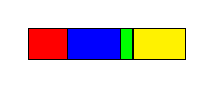
\begin{tikzpicture} 
\draw[fill=red] (0cm, 0cm) rectangle (0.502cm, .4cm);
\draw[fill=blue] (0.502cm, 0cm) rectangle (1.174cm, .4cm);
\draw[fill=green] (1.174cm, 0cm) rectangle (1.33cm, .4cm);
\draw[fill=yellow] (1.33cm, 0cm) rectangle (2cm, .4cm);
\end{tikzpicture}
\\ \cline{2-3}
\rule[-3ex]{0cm}{7ex} $\Delta\ell =$  6.31 & r-ad \hspace{0cm} \parbox{1cm}{\hfill $q^{MP}$ \ $q^M, q^P$} & \parbox{2cm}{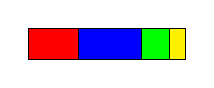
\begin{tikzpicture} 
\draw[fill=red] (0cm, 0cm) rectangle (0.636cm, .4cm);
\draw[fill=blue] (0.636cm, 0cm) rectangle (1.434cm, .4cm);
\draw[fill=green] (1.434cm, 0cm) rectangle (1.798cm, .4cm);
\draw[fill=yellow] (1.798cm, 0cm) rectangle (2cm, .4cm);
\end{tikzpicture}
\\[-1.3ex]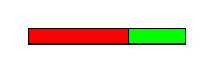
\begin{tikzpicture} 
\draw[fill=red] (0cm, 0cm) rectangle (1.274cm, .2cm);
\draw[fill=blue] (1.274cm, 0cm) rectangle (1.274cm, .2cm);
\draw[fill=green] (1.274cm, 0cm) rectangle (2cm, .2cm);
\draw[fill=yellow] (2cm, 0cm) rectangle (2cm, .2cm);
\end{tikzpicture}
\\[-2ex]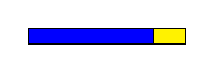
\begin{tikzpicture} 
\draw[fill=red] (0cm, 0cm) rectangle (0cm, .2cm);
\draw[fill=blue] (0cm, 0cm) rectangle (1.594cm, .2cm);
\draw[fill=green] (1.594cm, 0cm) rectangle (1.594cm, .2cm);
\draw[fill=yellow] (1.594cm, 0cm) rectangle (2cm, .2cm);
\end{tikzpicture}
}\\ \hline 
\rule[-1ex]{0cm}{4ex}Kidd & ad \hspace{1cm} \parbox{.5cm}{$q$ \\[-1.3ex] \mbox{}}& 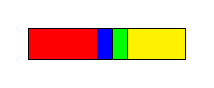
\begin{tikzpicture} 
\draw[fill=red] (0cm, 0cm) rectangle (0.876cm, .4cm);
\draw[fill=blue] (0.876cm, 0cm) rectangle (1.066cm, .4cm);
\draw[fill=green] (1.066cm, 0cm) rectangle (1.26cm, .4cm);
\draw[fill=yellow] (1.26cm, 0cm) rectangle (2cm, .4cm);
\end{tikzpicture}
 \\ \cline{2-3}
\rule[-3ex]{0cm}{7ex}$\Delta\ell =$  1.52  & r-ad \hspace{0cm} \parbox{1cm}{\hfill $q^{MP}$ \ $q^M, q^P$} & \parbox{2cm}{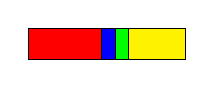
\begin{tikzpicture} 
\draw[fill=red] (0cm, 0cm) rectangle (0.932cm, .4cm);
\draw[fill=blue] (0.932cm, 0cm) rectangle (1.106cm, .4cm);
\draw[fill=green] (1.106cm, 0cm) rectangle (1.268cm, .4cm);
\draw[fill=yellow] (1.268cm, 0cm) rectangle (2cm, .4cm);
\end{tikzpicture}
\\[-1.3ex]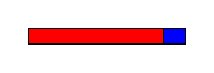
\begin{tikzpicture} 
\draw[fill=red] (0cm, 0cm) rectangle (1.716cm, .2cm);
\draw[fill=blue] (1.716cm, 0cm) rectangle (2cm, .2cm);
\draw[fill=green] (2cm, 0cm) rectangle (2cm, .2cm);
\draw[fill=yellow] (2cm, 0cm) rectangle (2cm, .2cm);
\end{tikzpicture}
\\[-2ex]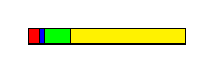
\begin{tikzpicture} 
\draw[fill=red] (0cm, 0cm) rectangle (0.146cm, .2cm);
\draw[fill=blue] (0.146cm, 0cm) rectangle (0.212cm, .2cm);
\draw[fill=green] (0.212cm, 0cm) rectangle (0.534cm, .2cm);
\draw[fill=yellow] (0.534cm, 0cm) rectangle (2cm, .2cm);
\end{tikzpicture}
}\\ \hline 
\end{tabular}} 

\vspace{2ex}\parbox{.5\textwidth}{\begin{tabular}{ll|r}
\multicolumn{3}{l}{HG03803, SAS, BEB}\\ \hline\rule[-1ex]{0cm}{4ex}EURO & ad \hspace{1cm} \parbox{.5cm}{$q$ \\[-1.3ex] \mbox{}}& 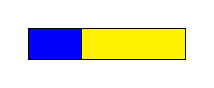
\begin{tikzpicture} 
\draw[fill=red] (0cm, 0cm) rectangle (0cm, .4cm);
\draw[fill=blue] (0cm, 0cm) rectangle (0.674cm, .4cm);
\draw[fill=green] (0.674cm, 0cm) rectangle (0.674cm, .4cm);
\draw[fill=yellow] (0.674cm, 0cm) rectangle (2cm, .4cm);
\end{tikzpicture}
\\ \cline{2-3}
\rule[-3ex]{0cm}{7ex} $\Delta\ell =$  1.01 & r-ad \hspace{0cm} \parbox{1cm}{\hfill $q^{MP}$ \ $q^M, q^P$} & \parbox{2cm}{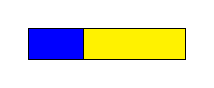
\begin{tikzpicture} 
\draw[fill=red] (0cm, 0cm) rectangle (0cm, .4cm);
\draw[fill=blue] (0cm, 0cm) rectangle (0.698cm, .4cm);
\draw[fill=green] (0.698cm, 0cm) rectangle (0.698cm, .4cm);
\draw[fill=yellow] (0.698cm, 0cm) rectangle (2cm, .4cm);
\end{tikzpicture}
\\[-1.3ex]\begin{tikzpicture} 
\draw[fill=red] (0cm, 0cm) rectangle (0cm, .2cm);
\draw[fill=blue] (0cm, 0cm) rectangle (0cm, .2cm);
\draw[fill=green] (0cm, 0cm) rectangle (0cm, .2cm);
\draw[fill=yellow] (0cm, 0cm) rectangle (2cm, .2cm);
\end{tikzpicture}
\\[-2ex]\begin{tikzpicture} 
\draw[fill=red] (0cm, 0cm) rectangle (0cm, .2cm);
\draw[fill=blue] (0cm, 0cm) rectangle (1.394cm, .2cm);
\draw[fill=green] (1.394cm, 0cm) rectangle (1.394cm, .2cm);
\draw[fill=yellow] (1.394cm, 0cm) rectangle (2cm, .2cm);
\end{tikzpicture}
}\\ \hline 
\rule[-1ex]{0cm}{4ex}Kidd & ad \hspace{1cm} \parbox{.5cm}{$q$ \\[-1.3ex] \mbox{}}& \begin{tikzpicture} 
\draw[fill=red] (0cm, 0cm) rectangle (0.108cm, .4cm);
\draw[fill=blue] (0.108cm, 0cm) rectangle (0.592cm, .4cm);
\draw[fill=green] (0.592cm, 0cm) rectangle (0.74cm, .4cm);
\draw[fill=yellow] (0.74cm, 0cm) rectangle (2cm, .4cm);
\end{tikzpicture}
 \\ \cline{2-3}
\rule[-3ex]{0cm}{7ex}$\Delta\ell =$  1.12  & r-ad \hspace{0cm} \parbox{1cm}{\hfill $q^{MP}$ \ $q^M, q^P$} & \parbox{2cm}{\begin{tikzpicture} 
\draw[fill=red] (0cm, 0cm) rectangle (0.116cm, .4cm);
\draw[fill=blue] (0.116cm, 0cm) rectangle (0.836cm, .4cm);
\draw[fill=green] (0.836cm, 0cm) rectangle (1.168cm, .4cm);
\draw[fill=yellow] (1.168cm, 0cm) rectangle (2cm, .4cm);
\end{tikzpicture}
\\[-1.3ex]\begin{tikzpicture} 
\draw[fill=red] (0cm, 0cm) rectangle (0.232cm, .2cm);
\draw[fill=blue] (0.232cm, 0cm) rectangle (0.232cm, .2cm);
\draw[fill=green] (0.232cm, 0cm) rectangle (0.894cm, .2cm);
\draw[fill=yellow] (0.894cm, 0cm) rectangle (2cm, .2cm);
\end{tikzpicture}
\\[-2ex]\begin{tikzpicture} 
\draw[fill=red] (0cm, 0cm) rectangle (0cm, .2cm);
\draw[fill=blue] (0cm, 0cm) rectangle (1.442cm, .2cm);
\draw[fill=green] (1.442cm, 0cm) rectangle (1.442cm, .2cm);
\draw[fill=yellow] (1.442cm, 0cm) rectangle (2cm, .2cm);
\end{tikzpicture}
}\\ \hline 
\end{tabular}}\parbox{.5\textwidth}{\begin{tabular}{ll|r}
\multicolumn{3}{l}{NA20864, SAS, GIH}\\ \hline\rule[-1ex]{0cm}{4ex}EURO & ad \hspace{1cm} \parbox{.5cm}{$q$ \\[-1.3ex] \mbox{}}& \begin{tikzpicture} 
\draw[fill=red] (0cm, 0cm) rectangle (0cm, .4cm);
\draw[fill=blue] (0cm, 0cm) rectangle (0.298cm, .4cm);
\draw[fill=green] (0.298cm, 0cm) rectangle (0.784cm, .4cm);
\draw[fill=yellow] (0.784cm, 0cm) rectangle (2cm, .4cm);
\end{tikzpicture}
\\ \cline{2-3}
\rule[-3ex]{0cm}{7ex} $\Delta\ell =$  0.87 & r-ad \hspace{0cm} \parbox{1cm}{\hfill $q^{MP}$ \ $q^M, q^P$} & \parbox{2cm}{\begin{tikzpicture} 
\draw[fill=red] (0cm, 0cm) rectangle (0cm, .4cm);
\draw[fill=blue] (0cm, 0cm) rectangle (0.38cm, .4cm);
\draw[fill=green] (0.38cm, 0cm) rectangle (1cm, .4cm);
\draw[fill=yellow] (1cm, 0cm) rectangle (2cm, .4cm);
\end{tikzpicture}
\\[-1.3ex]\begin{tikzpicture} 
\draw[fill=red] (0cm, 0cm) rectangle (0cm, .2cm);
\draw[fill=blue] (0cm, 0cm) rectangle (0cm, .2cm);
\draw[fill=green] (0cm, 0cm) rectangle (0cm, .2cm);
\draw[fill=yellow] (0cm, 0cm) rectangle (2cm, .2cm);
\end{tikzpicture}
\\[-2ex]\begin{tikzpicture} 
\draw[fill=red] (0cm, 0cm) rectangle (0cm, .2cm);
\draw[fill=blue] (0cm, 0cm) rectangle (0.762cm, .2cm);
\draw[fill=green] (0.762cm, 0cm) rectangle (2cm, .2cm);
\draw[fill=yellow] (2cm, 0cm) rectangle (2cm, .2cm);
\end{tikzpicture}
}\\ \hline 
\rule[-1ex]{0cm}{4ex}Kidd & ad \hspace{1cm} \parbox{.5cm}{$q$ \\[-1.3ex] \mbox{}}& \begin{tikzpicture} 
\draw[fill=red] (0cm, 0cm) rectangle (0.106cm, .4cm);
\draw[fill=blue] (0.106cm, 0cm) rectangle (0.246cm, .4cm);
\draw[fill=green] (0.246cm, 0cm) rectangle (0.878cm, .4cm);
\draw[fill=yellow] (0.878cm, 0cm) rectangle (2cm, .4cm);
\end{tikzpicture}
 \\ \cline{2-3}
\rule[-3ex]{0cm}{7ex}$\Delta\ell =$  0.95  & r-ad \hspace{0cm} \parbox{1cm}{\hfill $q^{MP}$ \ $q^M, q^P$} & \parbox{2cm}{\begin{tikzpicture} 
\draw[fill=red] (0cm, 0cm) rectangle (0.156cm, .4cm);
\draw[fill=blue] (0.156cm, 0cm) rectangle (0.312cm, .4cm);
\draw[fill=green] (0.312cm, 0cm) rectangle (1.146cm, .4cm);
\draw[fill=yellow] (1.146cm, 0cm) rectangle (2cm, .4cm);
\end{tikzpicture}
\\[-1.3ex]\begin{tikzpicture} 
\draw[fill=red] (0cm, 0cm) rectangle (0.314cm, .2cm);
\draw[fill=blue] (0.314cm, 0cm) rectangle (0.624cm, .2cm);
\draw[fill=green] (0.624cm, 0cm) rectangle (0.624cm, .2cm);
\draw[fill=yellow] (0.624cm, 0cm) rectangle (2cm, .2cm);
\end{tikzpicture}
\\[-2ex]\begin{tikzpicture} 
\draw[fill=red] (0cm, 0cm) rectangle (0cm, .2cm);
\draw[fill=blue] (0cm, 0cm) rectangle (0cm, .2cm);
\draw[fill=green] (0cm, 0cm) rectangle (1.668cm, .2cm);
\draw[fill=yellow] (1.668cm, 0cm) rectangle (2cm, .2cm);
\end{tikzpicture}
}\\ \hline 
\end{tabular}} 

\vspace{2ex}